\chapter{Sistemas de control de versiones}

Un sistema de control de versiones es un sistema que nos permite tener un histórico de las modificaciones que sufre un fichero a lo largo del tiempo.

Si pensamos en un documento, un ciclo de vida con modificaciones puede ser:

\begin{enumerate}
    \item Crear el documento.
    \item Correcciones.
    \item Cambios gramaticales.
    \item Modificar colores de los encabezados.
    \item Añadir logo de la compañía.
    \item Modificaciones finales.
\end{enumerate}

Los sistemas de control de versiones pueden controlar las modificaciones de cualquier tipo de fichero, pero son especialmente útiles cuando se trata con ficheros de tipo texto, como código fuente, documentos tipo texto/markdown, imágenes de tipo vectorial svg...




\chapter{Un poco de historia}

Aunque ha habido, y siguen existiendo, muchos sistemas de control, vamos a enumerar unos pocos que han tenido cierta relevancia en el mundo del software:

\begin{itemize}
    \item \textbf{CVS}: En inglés \textit{concurrent versions systems}, creado en el año 1990, comenzó como un \textit{frontend} de un sistema de versiones anterior (llamado RCS). Añadió funcionalidades sobre RCS hasta que se consideró un sistema propio. En el mundo del software libre ganó muchos adeptos a pesar de que era complicado de utilizar y tenía ciertas carencias y fallos.

    \item \textbf{Subversion}: Apareció en el año 2000 con la intención de ser parecido a CVS pero tratando de corregir fallos del anterior y añadirle características que carecía. Hace uso de un sistema basado en un repositorio central al que se envían los cambios. Debido a las mejoras que tenía, y la aparición del portal \href{https://sourceforge.net/}{Sourceforge}, se vuelve muy utilizado y prácticamente como el sistema principal del Sofware Libre.

    \item \textbf{Bitkeeper}: Es un sistema de control de versiones distribuido originalmente como software privativo, pero que permitió hacer uso de manera gratuita a los desarrolladores del kernel Linux (hasta el año 2005). Los desarrolladores del kernel Linux adoptaron esta solución porque ya desde 1998 \href{https://lkml.org/lkml/1998/9/30/122}{estaban teniendo problemas}, y no podían adoptar un sistema centralizado.

    \item \textbf{GNU Bazaar}: Creado en 2005 por la empresa Canonical (creadores de Ubuntu), es un sistema de control de versiones distribuido. La idea era impulsarlo como gestor del código utilizado en Ubuntu.

    \item \textbf{Git}: Creado por Linus Torvalds en 2005 debido al cambio de licencia de Bitkeeper. Decidió crearlo debido a que quería un sistema distribuido tal como usaba Bitkeeper, pero ninguno de los que había en ese momento le satisfacía.
\end{itemize}

\begin{center}
    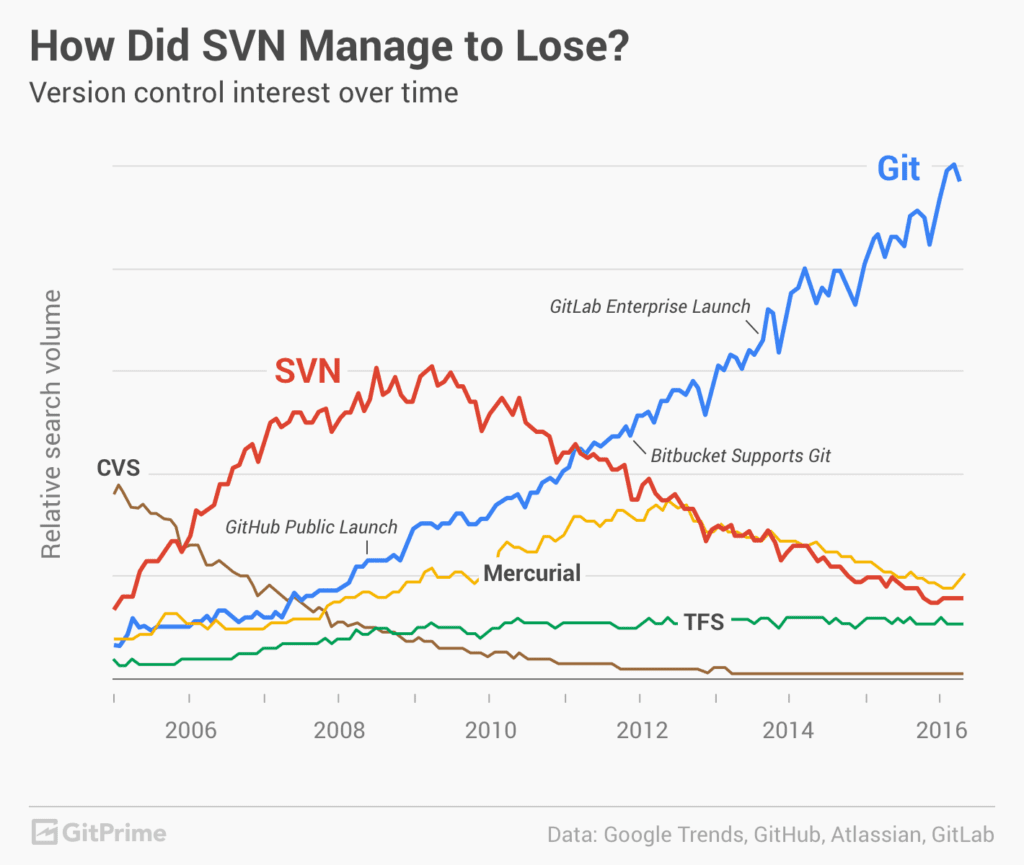
\includegraphics[frame,width=0.65\linewidth]{gitgraph.png}
    \captionof{figure}{Interés por los distintos sistemas de control de versiones. \href{https://fahadhussaincs.blogspot.com/2018/07/git-vs-github-understanding-and.html}{Fuente}.}
\end{center}

Wikipedia tiene una página donde se puede visualizar una \href{https://en.wikipedia.org/wiki/Comparison_of_version-control_software}{comparativa de distintos sistemas de control de versiones}. En ella se comparan información general, licencias, características, ... Es una buena manera de conocer otros sistemas aparte de los nombrados previamente.


\chapter{Características habituales}

Aunque cada sistema de control de versiones es diferente, todos tienen las siguientes características:

\begin{itemize}
    \item Comprobar el estado de los ficheros: si han sido modificados.
    \item Identificar cada cambio de una manera única.
    \item Conocer quién ha realizado las modificaciones que han sufrido los ficheros.
    \item Visualizar la diferencias que ha habido entre versiones en los ficheros.
    \item Volver atrás a una versión concreta del fichero, o de todo el proyecto.
    \item Tener un sistema de etiquetas para nombrar un estado concreto del proyecto.
\end{itemize}

Más adelante, con el ejemplo de Git, veremos qué significa cada una de esas características y cómo se realiza en Git.

\chapter{Tipos de sistemas de control de versiones}

Dentro de los sistemas de control de versiones se pueden diferenciar dos tipos cuando hablamos de cómo se interactúa y de cómo se almacena el histórico de todos los cambios.

\section{Centralizado}

El sistema centralizado era el más utilizado hasta la llegada y expansión de Git. Sistemas centralizados son CVS y Subversion.

El histórico de las modificaciones de nuestro repositorio se encontraba centralizado en un servidor. Cada vez que un usuario quería comprobar los cambios que había realizado, crear un commit, o volver a una versión anterior del proyecto \textbf{necesitaba realizar una conexión con el servidor central}.

\begin{center}
    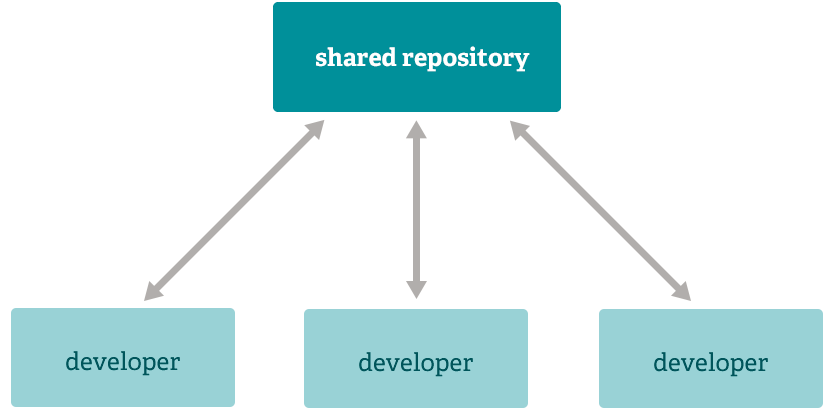
\includegraphics[width=0.65\linewidth]{workflow-a.png}
    \captionof{figure}{Arquitectura centralizada. \href{https://git-scm.com/about/distributed}{Fuente}.}
\end{center}

Esto suponía que era necesario tener siempre acceso a internet, y aparte, que para realizar pequeñas acciones cotidianas necesitases esperar a la respuesta del servidor.

Tampoco se podía saber si alguien había realizado modificaciones en el código hasta que no se intentasen subir nuevas modificaciones. De haber modificaciones y no tenerlas en la copia de trabajo local, había que resolver el conflicto, pudiendo dejar el servidor central en estado bloqueado.


\section{Distribuido}
Los sistemas de control de versiones distribuidos siguen la filosofía de que en cada copia de trabajo existen todos los datos, metadatos y el histórico completo de modificaciones que ha tenido el proyecto desde el inicio de los tiempos.

Gracias a eso, permite hacer uso del trabajo \textit{offline}, no necesitando la conexión a internet hasta que no nos interese subir los cambios realizados a un repositorio donde el resto de desarrolladores puedan acceder.

También es posible crear ramas locales, comprobar cómo ha evolucionado el proyecto, realizar \textit{diffs}... sin necesidad de realizar ningún tipo de conexión, por lo que estos cambios se realizan en local \textbf{mejorando la velocidad de trabajo}.

Trabajando de esta manera, también \textbf{nos permite centrarnos en las características que estamos realizando}, dejando para más adelante la posibilidad de que existan conflictos.

Por otro lado, el flujo de trabajo puede variar entre proyectos, y dentro de nuestro repositorio podemos tener distintos orígenes de los que obtener cambios. Un ejemplo de sistema distribuido:

\begin{center}
    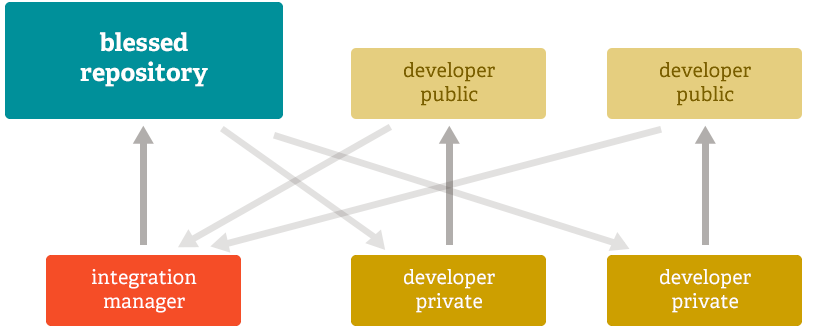
\includegraphics[width=0.65\linewidth]{workflow-b.png}
    \captionof{figure}{\textit{Workflow} distribuido. \href{https://git-scm.com/about/distributed}{Fuente}.}
\end{center}

En los sistemas distribuidos podemos hacer que el sistema de control de versiones se adapte a nuestra manera de trabajar, y no al revés.

\chapter{Glosario}
A la hora de utilizar un sistema de control de versiones tenemos que conocer cierta nomenclatura que es habitual. Es importante conocer estas palabras para identificar a qué términos nos estamos refiriendo.

Como son palabras utilizadas por los propios sistemas de control de versiones en sus clientes de línea de comandos (o en interfaces gráficas), se ha decidido mantener en inglés.


\begin{description}[style=nextline]
    \item[Blame] Comprobar el autor y la revisión de la última vez que se modificó una línea de un documento. En inglés \textit{blame} significa culpar/acusar.
    \item[Branch] Los sistemas de control de versiones nos permiten crear ramificaciones (temporales o perpetuas) partiendo de una versión concreta.
    \item[Checkout] Es utilizado para poner el repositorio local en una revisión concreta del histórico.
    \item[Clone] Clonar significa crear un repositorio obteniendo todas las revisiones de otro repositorio.
    \item[Commit] Puede tener dos acepciones:
    \begin{itemize}
        \item Como nombre: Un “\textbf{\textit{commit}}” (o revisión), es el conjunto de modificaciones que se empaquetan conjuntamente. Un “commit” muestra las modificaciones realizadas respecto al commit anterior.

        Los commits deberían llevar modificaciones que tengan que ver entre sí y tratando de que sea código válido.
        \item Como verbo: Hacer un “commit”, o “\textit{\textbf{commitear}}”, es la acción de empaquetar modificaciones de nuestra copia de trabajo, para crear un “\textit{commit}”, o revisión, que va a pertenecer al histórico del proyecto.
    \end{itemize}
    \item[Origin] En sistemas de control de versiones distribuidos, es el nombre del repositorio remoto “central”.
    \item[Pull] Obtener y aplicar en el repositorio local todos los commits desde un repositorio remoto.
    \item[Push] Enviar los commits creados en local que no están en el repositorio remoto “central”.
    \item[Repository] Puede tener distintas acepciones dependiendo del sistema de control de versiones que estemos utilizando. Es la estructura de directorios y ficheros (junto con su metadata) en el que guardamos el proyecto que nos interesa versionar. En sistemas distribuidos, tanto la copia local como la remota se denominan repositorios.
    \item[Tag] Una etiqueta es la manera de darle un nombre que podemos identificar de manera “humana” a una revisión concreta. Normalmente se usa para indicar las versiones del software: v1.0, v1.5, ...
    \item[Working copy] Es la copia local de un repositorio, en un momento específico del tiempo o revisión.
\end{description}